
\scanpage{62}
\mspage{18}
Il faudrait expliciter un \uline{petit} théorème de dévissage préliminaire, qui dira qu'à équivalence près (définie à isom. uniques près)
$S_*\mathcal TD_{\mathrm{top}}^\pm$,
\inserted{avec le foncteur $\Gamma$ dans $(\mathrm{Gr.pond.rep})$ et $\chi$ dans $[\pm1]$, et}
avec les opérations élémentaires $1^\circ$ à $7^\circ$ (ou leurs variantes composées simultanées) se réconstitue par la connaissance des groupoïdes et foncteurs suivants
\margin{\uline{à l'exception de $4^\circ$ et $5^\circ$}}

\deleted{\diagram{\begin{tikzcd}[ampersand replacement=\&,row sep=large,column sep=large]
S_1\mathcal T_{g,\nu}^{\deleted{\unsure{0}}\pm}\arrow[r]\arrow[d]
\&{[\pm1]}\\
\unsure{\mathrm{Ens}(\nu)}
\end{tikzcd}}}
\deleted{\diagram{\begin{tikzcd}[ampersand replacement=\&]
\&\mathcal T_{g,\nu}^{\pm}\arrow[dl]\\
{}\&
\end{tikzcd}}}

$(*)$\quad
\diagram{\fbox{\begin{tikzcd}[ampersand replacement=\&,column sep=large]
S_1\mathcal T_{g,\nu}^\pm\arrow[r]
\&\mathcal T_{g,\nu}^\pm\arrow[r]
\&(\mathrm{Ens}(\nu)\times[\pm1])
\end{tikzcd}}}
\margin{(on \unsure{siglera|notera} $S\mathcal T_{g\nu}^\pm$)}
\deleted{\unsure{$\varnothing$}}

$S_1\mathcal T_{g,\nu}^\pm$ désigne le sous-groupoïde de $S_*\mathcal T_{\mathrm{top}}^\pm$ formé des $(X,R)$ tels que $X$ soit connexe de genre $g$, $\operatorname{card}\pi_0\partial X=\nu$, et $\operatorname{card}R\cap C_a=1$ (pour tout $a\in\pi_0\partial X$ --- i.e. le graphe \inserted{bipondéré} de
$\deleted{\unsure{\mathcal T_{g,\nu}}}(X,\underset{\Vert\,\partial X}{\widetilde\Sigma},R)$ est isom. à
\figure{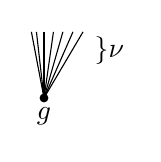
\begin{tikzpicture}[scale=.8]
\fill (0,0) circle(2pt);
\node[below] at (0,0) {$g$};
\foreach \x in {-.2,-.12,0,.15,.3,.46,.62}{\draw (0,0)--(\x,1.05);}
\node[right] at (.65,.75) {$\}\nu$};
\end{tikzpicture}}
toutes ces arêtes (libres) sont de poids 1

et $\mathcal T_{g,\nu}^\pm$ est défini de façon correspondante, via les $(X,\varnothing,\varnothing)$ où $X$ de type $g,\nu$.

\margin{Ça ne suffit pas tout à fait, pour reconstituer les opérations Notamment les opérations
\textcircled{$4^\circ$} (qui \unsure{demande} des \deleted{\unsure{liens}} \inserted{\unsure{``ou''}} \unsure{structures} \unsure{$\mathcal T_{g,\infty}$}) et \textcircled{$5^\circ$}}
\mspage{61}
